\documentclass[answers]{exam}

%% Language and font encodings
\usepackage{CJKutf8}
\usepackage[english]{babel}
\usepackage[utf8]{inputenc}
\usepackage[T1]{fontenc}
\usepackage{natbib}

%% Color
\usepackage[dvipsnames]{xcolor}

%% Sets page size and margins
\usepackage[a4paper,margin=2cm]{geometry}

%% Useful packages
\usepackage{amsmath}
\usepackage{graphicx}
\usepackage{paralist}
\setlength\FrameSep{4pt}

\begin{document}
\begin{CJK}{UTF8}{min}
\begin{questions}

%%%%%%%%%%%%%%%%%%%%%%%%%
\question[10]{Copy your code comments here.}
\begin{framed}
\begin{compactenum}[A.]
  \item
    Create \texttt{nlayers\_enc} encoding layers using \texttt{add\_link}. There
    are two loops for adding layers because we create one encoder to pass over
    the sentence in order, and one to pass over the sentence in reverse order.
  \item
    The encoding of a sentence is a matrix, each column of which is the
    concatenation of the hidden states of the forward and the backward encoder
    LSTMs at that position. Since both the LSTMs are sized \texttt{n\_units},
    the concatenation of these two hidden states is \texttt{2*n\_units}.
  \item
    The method \texttt{set\_decoder\_state} will feed the encoder output into
    the decoder. The initial implementation takes the cell states and hidden
    state from the final LSTM of the encoder, and feeds them into the first LSTM
    of the decoder.
  \item
    We are performing two encode operations because we are stepping through the
    sentence forwards and backwards at the same time -- see the call to
    \texttt{zip} above -- and we are encoding the `forwards' word using the
    forwards encoder, and the backwards word using the backwards encoder.
  \item
    Let us assume we have a vector $x$ of activations $[0.8, 0.6, 0.3]$,
    with each position in the vector corresponding to a word in
    the output vocabulary. Let us also assume we have a scalar $t$, say $2$,
    which represents the true index of the word to be generated.
    We take the softmax of $x$ to get a probability distribution, and we turn
    $t$ into a one-hot vector (also a probability distribution).
    We then compute the loss as the cross-entropy over these two distributions:
    $-\sum_{i} x(i) \log{t(i)}$. In our running example, this would work out to
    be $\pm 1.39$. This measures how close the network got to the true answer.
  \item
    The \texttt{add\_hook} function adds some code which is to be executed right
    after the computation of the gradient. The \texttt{GradientClipping}
    function will scale gradients down when their L2 norm goes over a certain
    threshold (here 5).
\end{compactenum}
\end{framed}


%%%%%%%%%%%%%%%%%%%%%%%%%
\question[10]{Examine the parallel data and answer questions. (Plots may appear in the appendix.)}
\begin{framed}
\begin{compactenum}[1.]
  \item
    When looking at figures \ref{fig:corr-toks} and \ref{fig:corr-chars}, it
    seems as if English is a more productive language (more `meaning' with fewer
    symbols) when we measure sentence length in tokens, and Japanese is more
    productive when we measure it in characters. There explanations for both
    these observations, which I'll go into in Q3.

    What our graphs do make clear, however, is that there is a linear
    correlation between sentence lengths in English and Japanese. This means
    that we can expect sentence length to change linearly when we translate,
    either as $|f| \approx 1.42|e|$ (tokens) or as $|f| \approx 0.42|e|$
    (characters).
  \item
    In total, there are 97643 and 143581 tokens in the English and Japanese
    data, respectively.
  \item
    There are 7217 and 8246 word types/unique tokens in the English and Japanese
    data, respectively.
  \item
    In the default implementation, the vocabulary size is 3713 for English and
    3949 for Japanese. This means that tokens of 3505 and 4298 token types will
    be replaced with \texttt{\_UNK}, assuming \texttt{\_UNK} is part of the
    vocabulary. These account for 3608 (3.82\%) and 4413 (3.28\%) tokens in the
    data.
  \item
    A vocabulary of 3713 tokens is \emph{really} small. When we look at the most
    common \texttt{\_UNK} words -- \texttt{users protest commerce irony hats} --
    we see that these are still quite common. While $\pm 3.5\%$ does not sound
    like a lot, it will probably cripple a large number of translations with
    \texttt{\_UNK} words. Furthermore, this will probably make \texttt{\_UNK}
    quite difficult for the network to translate, at it will occur in huge
    number of syntactic positions.
    The differences in sentence length seems linear enough not to be a big
    problem.
  \end{compactenum}
\end{framed}


%%%%%%%%%%%%%%%%%%%%%%%%%
\question[10]{What language phenomena might influence what you observed above?}
\begin{framed}
  Our two measures for sentence length seem to contradict one another. Let's
  look at Japanese to see why:
  \begin{compactitem}
  \item {\it High productivity using characters.}
    Japanese uses logograms, and each logogram corresponds to one or more
    syllables. Thus, each character in Japanese can carry far more information
    than in English.
  \item {\it Low productivity using tokens.}
    Japanese also uses post-positional clitics to mark e.g.\ subjects and
    objects~\citep{Hinds-1986}, which are treated as separate tokens.
    Many uses of these clitics, e.g.\ topic, subject, object, are marked in
    English using word order and some vestigial cases, neither of which adds
    tokens.
    Making matters worse, the tokeniser for Japanese seems to treat each
    hiragana as its own token, meaning long and common verb endings such as
    `-します' are treated as three separate
    tokens~\citep{Minna-1998}.
  \end{compactitem}
\end{framed}


%%%%%%%%%%%%%%%%%%%%%%%%%
\question[10]{Answers to questions about sampling, beam search, and dynamic programming.}
\begin{framed}
\begin{compactenum}[1.]
\item
  It seems that the argmax version has a bias towards generating more common
  words. For instance, have a look at the translation below:

  \begin{tabular}{ll}
    source    & 皮肉 な 笑い を 浮かべ て 彼 は 私 を 見つめ た 。\\
    reference & he stared at me with a satirical smile .\\
    baseline  & i gave him him he him him him . \_EOS\\
  \end{tabular}

  The sampling version ``solves'' this problem to the extend that it is a lot
  less common. Unfortunately, this does not mean its translations are better.

  \begin{tabular}{ll}
    sampling & he gave him from his coming he much . \_EOS\\
    sampling & i came him him to borrow him him . \_EOS\\
    sampling & i gave him him for they died job \_EOS
  \end{tabular}
  \item
    How did we implement beam search for the phrase-based model? The idea was
    that each phrase in the output would correspond to a phrase on the input,
    and that these may be permuted in some way.
    However, our NMT model no longer \emph{really} has this property. It simply
    consumes a bunch of words, and then produces out a bunch of words, with no
    obvious relation between an output phrase and an input phrase.

    So, what can we do? We could use beam search to search all possible
    output phrases. When decoding, I have access to a list of all possible next
    words (namely, the vocabulary) and a score for each possible next word
    (namely, the log of that word's probability according to the network's
    output distribution). A naive implementation could simply branch, trying
    each possible word as the next word, and scoring the generated sentences
    using the sum of the log-probabilities.
    From here, we can add the beam search heuristic, e.g.\ at each step, we only
    keep the $k$ most promising sentences. We simply keep expanding the $k$ best
    sentences until they produce an \texttt{\_EOS} token (or run into the
    \texttt{MAX\_PREDICT\_LEN} setting).
  \item
    We cannot implement dynamic programming for the above model, because we have
    no notion of when translations are sharing work. This was also discussed
    above: we don't know what phrases in the source language correspond to which
    phrases in the target language. We only know that the NMT model has chosen
    to generate some phrase. Therefore we cannot say that some partial
    translation is better than another partial translation which translates the
    same source words, because we don't know which source words a partial
    translation translates.

    Furthermore, discounting the \texttt{MAX\_PREDICT\_LEN} setting, there is no
    way to know when translations are done, or how long the translations will
    be, because we are basically waiting for the \texttt{\_EOS} token to be
    predicted, and there is no knowing when that will happen.
\end{compactenum}
\end{framed}


%%%%%%%%%%%%%%%%%%%%%%%%%
\question[10]{Experiment with changes to the model, and explain results.}
\begin{framed}
  For this experiment, I trained a model with a 2-layer encode, and a 2-layer
  decoder. I compare this models after 10 epochs of training, to the provided
  baseline, as well as throughout their training with two baselines which I
  trained specifically for this purpose. See figure~\ref{fig:bleu-pplx}.

  This model did not do well. It managed to find new lows in its BLEU score, and
  new highs in perplexity. It is hard to compare the translations generated by
  the baselines with those generated by the new model as both are, in fact,
  terrible. However, some of the translations that \emph{almost} worked under
  our original baseline, bear no resemblance to the reference translation under
  the 2-layer model:

  \begin{tabular}{ll}
    source    & 宿題 は もう 終わ っ た の で す か 。\\
    reference & have you finished your homework already ? \_EOS  \\
    baseline  & have you finished your homework homework ? \_EOS \\
    2-layer   & where did you rain ? ? \_EOS
  \end{tabular}

  However, the model still learns some very basic features of Japanese. For
  instance, it consistently translates the question particle か as a question
  mark, but does not translate other occurrences of か as question marks.
\end{framed}


%%%%%%%%%%%%%%%%%%%%%%%%%
\question[10]{Implement dropout, and explain the results.}
\begin{framed}
  For this experiment, I trained two models with dropout as described
  by~\citet{Zaremba-2014}, with ratios of $0.5$ (the default value) and $0.2$
  (the recommended value). Once again, I will compare these models to the
  original baseline and the two which I trained myself. See
  figure~\ref{fig:bleu-pplx}.

  Dropout is a technique which randomly zeros out some connections, and
  therefore these two experiments might simply have been unlucky.
  That being said, we found that both our models using dropout perform worse on
  the BLEU score, losing between $4.6$ and $0.26$ points.
  As a minor consolation, both models with dropout maintain a fairly consistent
  perplexity throughout training, where the perplexity of the baselines
  skyrockets, almost doubling in the span of $10$ epochs.

  Once again, it is hard to compare the translations generated by the baselines
  with those generated by the models with dropout, as both are still terrible.
  However, if looking at my favorite translation, we find that again, the models
  with dropout mess up the only thing the baseline had going for it:

  \begin{tabular}{ll}
    source         & 宿題 は もう 終わ っ た の で す か 。\\
    reference      & have you finished your homework already ? \_EOS  \\
    baseline       & have you finished your homework homework ? \_EOS \\
    dropout($0.5$) & where did you you finish your ? ? \_EOS \\
    dropout($0.2$) & where did you you a ? ? ? \_EOS
  \end{tabular}

  Remarkably, the dropout($0.5$) model \emph{does} still generate the word
  ``finish''. Furthermore, looking at the remainder of the sentences, the
  dropout($0.5$) model still accurately translates the question particle か.
  Worryingly, the dropout($0.2$) model no longer translates all occurrences of
  か correctly. When looking at the scores, the seemingly better performance of
  dropout($0.5$) looks like a quirk of these examples, though I have found no
  reason to support this decision. Really, though, both are pretty bad.

  (While it is irrelevant, it is interesting to note that both the 2-layer model
  and the dropout model choose to translate the source using the phrase ``where
  did you''.) 
\end{framed}


%%%%%%%%%%%%%%%%%%%%%%%%%
\question[20]{Implement attention. This question will be evaluated on the basis of your code.}

\question[10]{Explain the results of implementing attention.}
\begin{framed}
  For this experiment, I trained two models with attention,
  after~\citet{Luong-2015}. One with, and one without dropout. Trusting BLEU
  and~\citet{Zaremba-2014}, I chose to use a ratio of $0.2$. Once again, I will
  compare these models to the original baseline and the two which I trained
  myself. See figure~\ref{fig:bleu-pplx}. 

  The attentional models are the first to best the baseline where BLEU is
  concerned, scoring $24.243$ and $25.089$ at their peaks, a good $4$ points
  higher than the best baseline. In terms of perplexity, it seems that my
  decision to use dropout payed off. The perplexity of the attentional model
  without dropout trails off into the sky, reaching the highest score I've found
  with a perplexity of $60.1225$ at epoch $10$. For the model \emph{with}
  dropout, however, the perplexity takes a dive after the second epoch, and
  stays low throughout, finishing on $28.5150$, the lowest recorded value for
  $10$ epochs of training.

  I was sad to see that my attentional model wasn't perfect, and in fact was
  still rather bad. However, looking over the sentences of the attentional
  model, I found that it more often than the baseline generated some of the
  expected words, for instance:

  \begin{tabular}{ll}
    source            & 丘 の 上 に 建 っ て い る 家 は とても 古 い 。\\
    reference         & the house which stands on the hill is very old .\\
    baseline          & it is well in is the the the . . \_EOS\\
    attention+dropout & house hill very on hill on hill the . \_EOS
  \end{tabular}

  And then there is the occasional gem, which captures the spirit, if not the
  exact phrasing, of the source:

  \begin{tabular}{ll}
    source            & ボブ は 読 み きれ な い ほど たくさん の 本 を 持 っ て い る 。\\
    reference         & bob has too many books to read . \\
    baseline          & bob is a a a a world . \_EOS\\
    attention+dropout & bob have books books books books books . \_EOS
  \end{tabular}
\end{framed}

%%%%%%%%%%%%%%%%%%%%%%%%%
\question[10]{Explain what you observe with attention. (Figures may appear in an appendix.)}
\begin{framed}
\emph{Your answer here}
\end{framed}
\end{questions}

\clearpage

\bibliography{main}
\bibliographystyle{apalike}

\begin{figure}
  \centering
  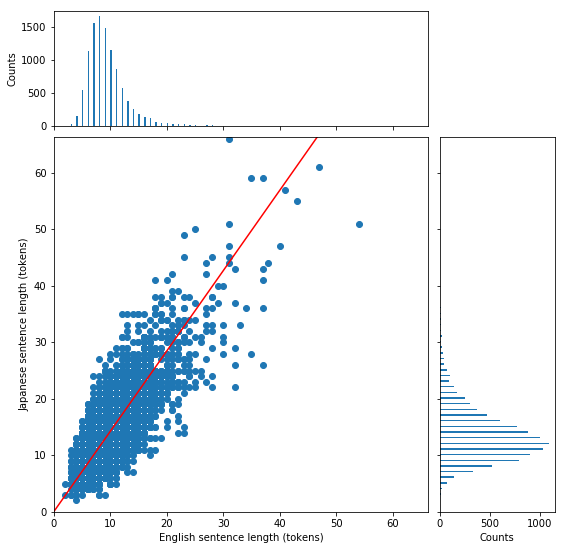
\includegraphics[width=\linewidth]{fig-corr-toks}
  \caption[Sentence lenths (tokens)]%
  {Distribution of and correlation between Japanese and English sentence lengths (tokens)}
  \label{fig:corr-toks}
\end{figure}

\begin{figure}
  \centering
  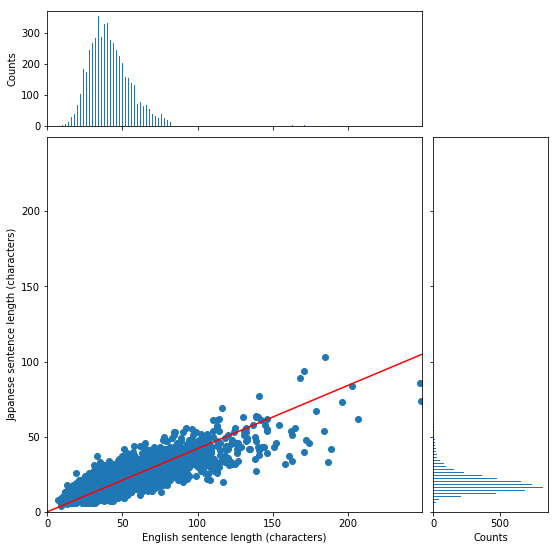
\includegraphics[width=\linewidth]{fig-corr-chars}
  \caption[Sentence lenths (characters)]%
  {Distribution of and correlation between Japanese and English sentence lengths (tokens)}
  \label{fig:corr-chars}
\end{figure}

\begin{figure}
  \centering
  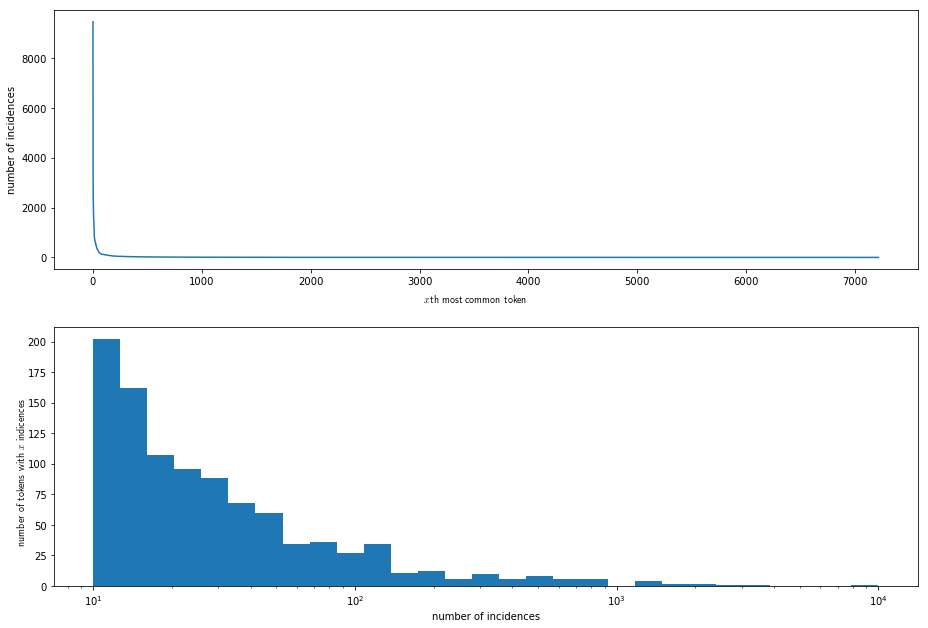
\includegraphics[width=\linewidth]{fig-toks-en}
  \caption{Counts for tokens and token types (English).}
  \label{fig:toks-en}
\end{figure}

\begin{figure}
  \centering
  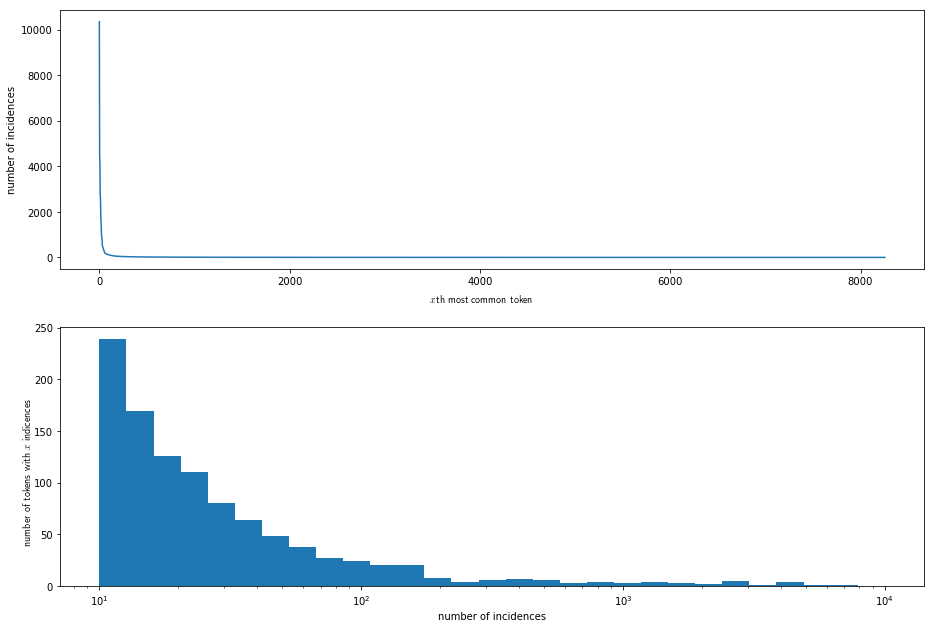
\includegraphics[width=\linewidth]{fig-toks-fr}
  \caption{Counts for tokens and token types (Japanese).}
  \label{fig:toks-fr}
\end{figure}

\begin{figure}
  \centering
  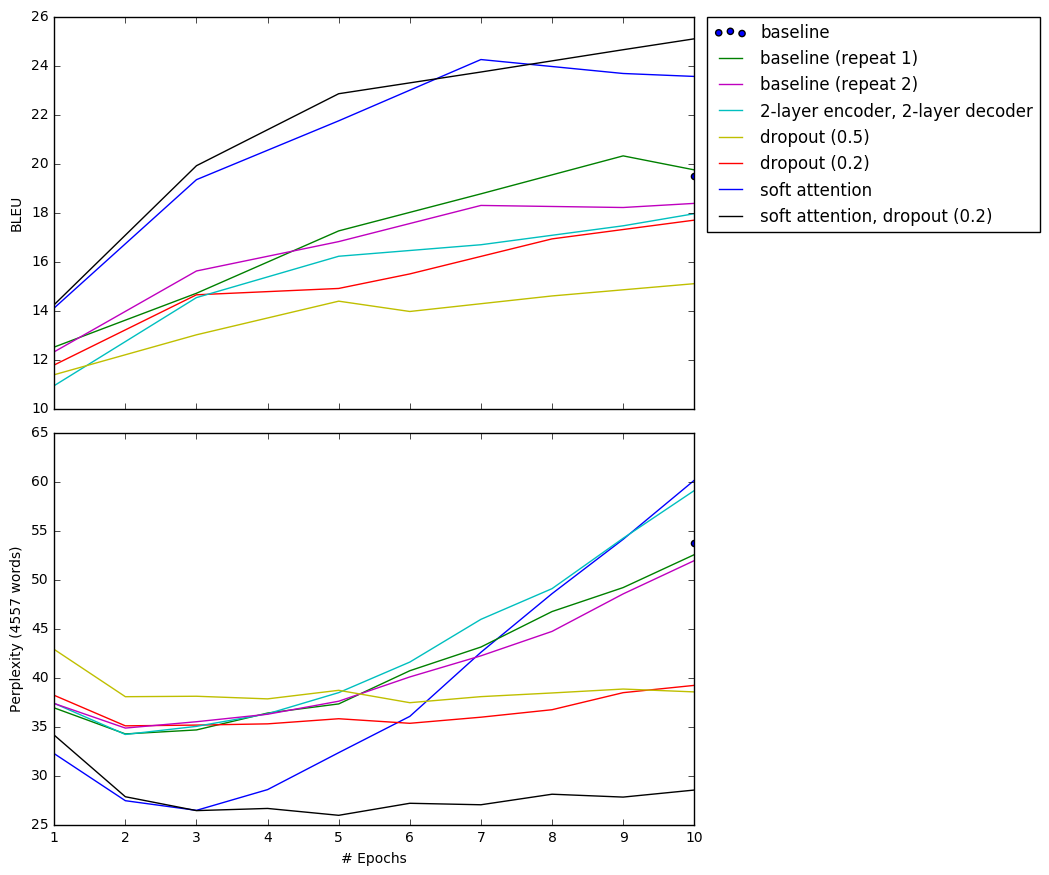
\includegraphics[width=\linewidth]{fig-bleu-pplx}
  \caption{BLEU and perplexity scores per epoch.}
  \label{fig:bleu-pplx}
\end{figure}

\end{CJK}
\end{document}